\section*{Abstract}
Feedback can improve either a model's parameters or the program that a model proposes. This study examines both processes through two reproducible, deliberately small experiments. First, a fixed Qwen2.5-0.5B policy was adapted with LoRA and clipped PPO on 512 arithmetic prompts. An NVIDIA A10 BF16 run completed 32 rollout batches, saved Actor and Critic adapters, and successfully reloaded the Actor. On the same 128 development-validation questions, greedy first-line accuracy increased from 117/128 (91.40625\%) to 122/128 (95.3125\%): five corrected answers with no newly incorrect answers. Second, an LLM-guided circle-packing search produced five valid online evaluations from seven saved proposals. Its best online sum of radii was 2.62001380699489; the global winner appeared during initialization rather than a later generation. Independent local execution of that unchanged program produced a valid but numerically different result, 2.6206092130170973, which is retained as a separate measurement. The study distinguishes training diagnostics from paired performance, and online scores from local verification. One seed, development-validation reuse, a manually stopped search and incomplete cost records limit broader conclusions. The main outcome is an inspectable account of feedback, execution and evidence in two optimization workflows.

\section{Introduction}
A scalar reward is useful only when the system can turn it into a controlled change. In policy learning, gradients modify trainable weights; in LLM-guided program search, execution results influence which source-code changes survive. These workflows share a feedback loop, while optimizing different objects with different measurements. Comparing their mechanisms is informative; comparing their raw scores would not be.

The first case studies whether a small language model can complete an adapter-only PPO workflow with a measurable, paired change on a fixed arithmetic task. The second studies how a hosted agent framework generates, evaluates and selects geometric-construction programs. Neither case introduces a new optimization algorithm. Together they provide source-linked experimental records, verified outputs and a practical separation between progress messages and completed outcomes.

\smallheading{Research questions}
\begin{enumerate}[label=\textbf{RQ\arabic*.}]
\item Under a fixed 512-prompt budget, does LoRA-PPO produce a saved, reloadable policy with a higher score on the same 128 arithmetic questions?
\item In a short LLM-guided program search, which candidates improve the measured objective, and what does independent geometric verification establish?
\end{enumerate}

The analysis follows the object that actually changes: adapter matrices in the first case and executable source code in the second. Figure~\ref{fig:feedback} summarizes this distinction. Throughout, numerical results are attributed to their own run, evaluator and execution environment. Historical failures remain available in the evidence package.

\par\noindent\begin{minipage}{\linewidth}
\begin{center}
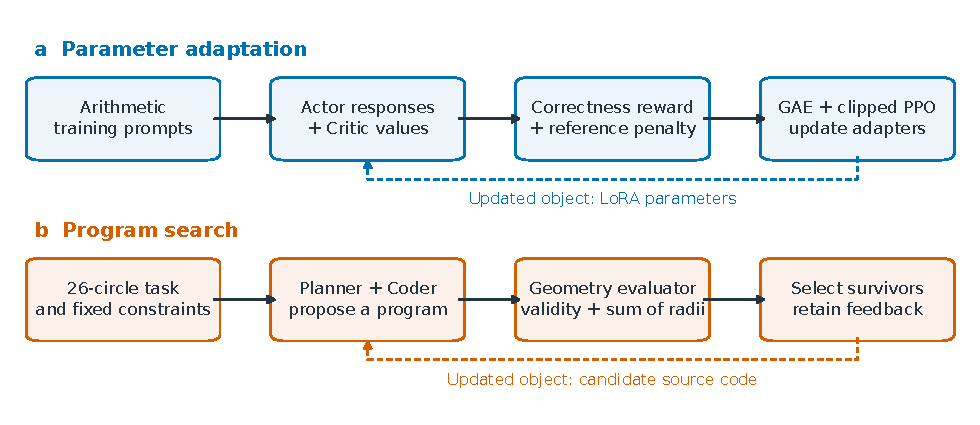
\includegraphics[width=166mm]{../../figures/feedback_mechanisms.pdf}
\end{center}
\figcaption{fig:feedback}{The two feedback mechanisms studied here. Policy optimization changes LoRA parameters through reward and gradient updates; program search changes candidate code through proposal, execution and selection. This is an explanatory mechanism diagram, not a measured comparison of efficiency.}
\end{minipage}\par

